%%%%%%%%%%%%%%%%%%%%%%%%%%%%%%%%%%%%%%%%%
% a0poster Portrait Poster
% LaTeX Template
% Version 1.0 (22/06/13)
%
% The a0poster class was created by:
% Gerlinde Kettl and Matthias Weiser (tex@kettl.de)
% 
% This template has been downloaded from:
% http://www.LaTeXTemplates.com
%
% License:
% CC BY-NC-SA 3.0 (http://creativecommons.org/licenses/by-nc-sa/3.0/)
%
%%%%%%%%%%%%%%%%%%%%%%%%%%%%%%%%%%%%%%%%%

%----------------------------------------------------------------------------------------
%	PACKAGES AND OTHER DOCUMENT CONFIGURATIONS
%----------------------------------------------------------------------------------------

\documentclass[a0,portrait]{a0poster}

\usepackage{multicol} % This is so we can have multiple columns of text side-by-side
\columnsep=100pt % This is the amount of white space between the columns in the poster
\columnseprule=3pt % This is the thickness of the black line between the columns in the poster
\usepackage{subfigure}
\usepackage[svgnames]{xcolor} % Specify colors by their 'svgnames', for a full list of all colors available see here: http://www.latextemplates.com/svgnames-colors

\usepackage{times} % Use the times font
%\usepackage{palatino} % Uncomment to use the Palatino font

\usepackage{graphicx} % Required for including images
\graphicspath{{figures/}} % Location of the graphics files
\usepackage{booktabs} % Top and bottom rules for table
\usepackage[font=small,labelfont=bf]{caption} % Required for specifying captions to tables and figures
\usepackage{amsfonts, amsmath, amsthm, amssymb} % For math fonts, symbols and environments
\usepackage{wrapfig} % Allows wrapping text around tables and figures

\begin{document}
	
	%----------------------------------------------------------------------------------------
	%	POSTER HEADER 
	%----------------------------------------------------------------------------------------
	
	% The header is divided into two boxes:
	% The first is 75% wide and houses the title, subtitle, names, university/organization and contact information
	% The second is 25% wide and houses a logo for your university/organization or a photo of you
	% The widths of these boxes can be easily edited to accommodate your content as you see fit
	
	\begin{minipage}[b]{0.75\linewidth}
		\veryHuge \color{NavyBlue} \textbf{Experiments on Metric Learning Methods} \color{Black}\\ % Title
		\huge \textbf{Shaoheng Liang and Yerong Li}\\[0.5cm] % Author(s)
	\end{minipage}
	
	\vspace{1cm} % A bit of extra whitespace between the header and poster content
	
	%----------------------------------------------------------------------------------------
	
	\begin{multicols}{2} % This is how many columns your poster will be broken into, a portrait poster is generally split into 2 columns
		
		%----------------------------------------------------------------------------------------
		%	ABSTRACT
		%----------------------------------------------------------------------------------------
		
		\color{SaddleBrown} % SaddleBrown color for the introduction
		
		\section*{Introduction}
		Metric learning is the task of learning a distance function on pair of objects. We experiment on three metric learning methods based on deep learning, including Siamese Network, Triplet Network and n-Tuple Network. The three approaches can be viewed as a framework that contains a set of network sharing parameters and a loss function integrating the outputs of the networks. The basic idea is to force the network to give shorter distance between similar instances and longer distance between dissimilar instances.
		
		We wrote a wrapper class for the network to hide the low-level implementation, and focus on the design of the high-level frameworks and loss functions. In our experiment on MNIST dataset and a classic network structure, Siamese Network has a mediocre performance while Triplet Network produces better embeddings. We are not able to make the original n-Tuple Network work. However, we have tested a few modified versions of it, which keep the framework unchanged but use different loss functions.
		
		%----------------------------------------------------------------------------------------
		%	OBJECTIVES
		%----------------------------------------------------------------------------------------
		
		\color{DarkSlateGray} % DarkSlateGray color for the rest of the content
		
		\section*{Main Objectives}
		
		\begin{enumerate}
			\item Implement a toolkit for experimenting deep metric learning methods.
			\item Experiment on Siamese, Triplet and n-Tuple Network and compare the results.
			\item Explore possible extensions to these networks.
		\end{enumerate}
		
		%------------------------------------------------
		
		\subsection*{Siamese Network}
		\begin{center}\vspace{1cm}
			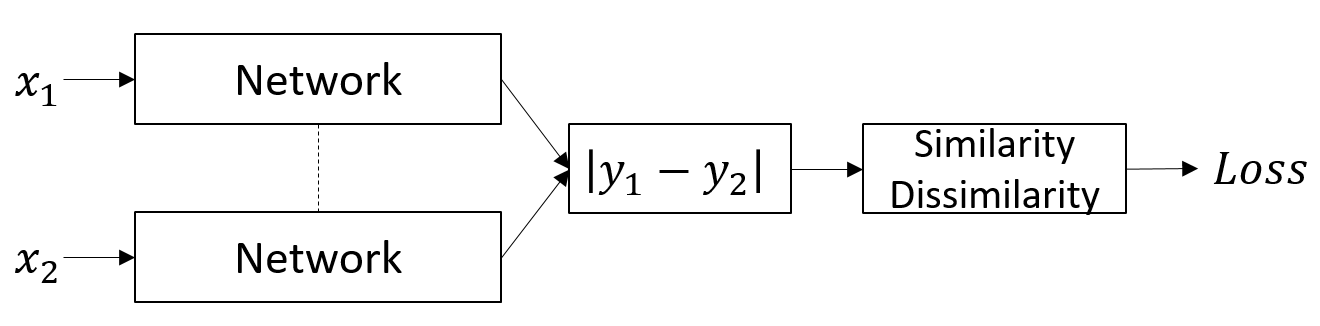
\includegraphics[width=0.7\linewidth]{../report_shaoheng/siamese_struct}
			\captionof{figure}{\color{Green} Structure of Siamese Network.}
		\end{center}\vspace{1cm}
		\begin{equation}
		Loss = (1-S)L_S(\lvert y_1 - y_2 \rvert) + S L_D(\lvert y_1 - y_2 \rvert)
		\end{equation}
		\begin{equation}
		L_S = \frac{1}{2}\lvert y_1 - y_2 \rvert^2
		\end{equation}
		\begin{equation}
		L_D = \frac{1}{2}\{max(0, m-|y_1-y_2|)\}^2
		\end{equation}
		\subsection*{Triplet Network}
		\begin{center}\vspace{1cm}
			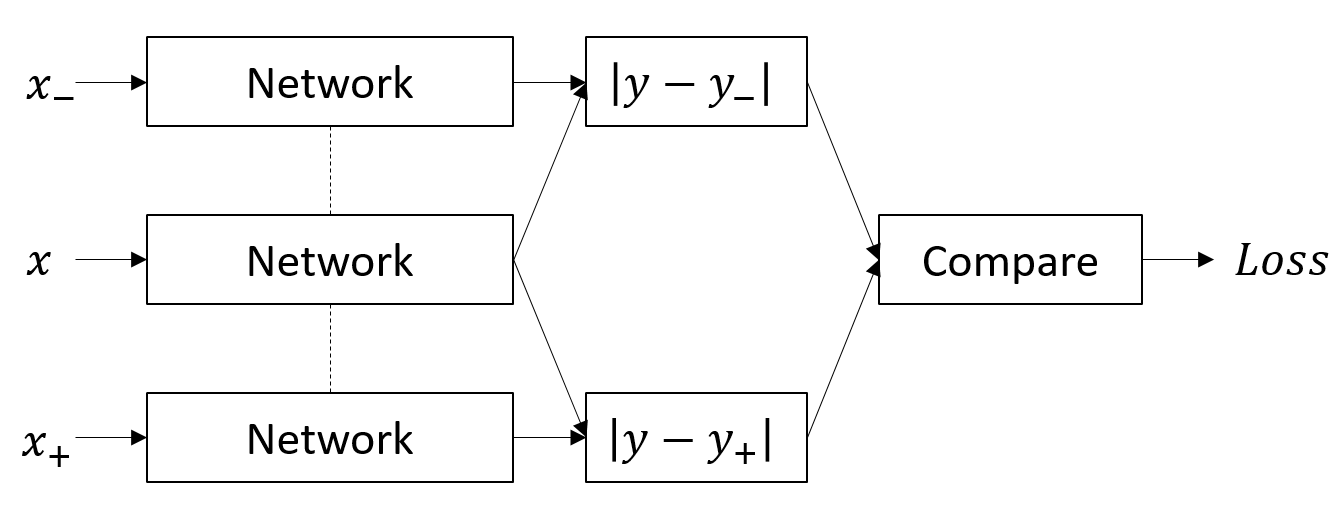
\includegraphics[width=0.7\linewidth]{../report_shaoheng/triplet_struct}
			\captionof{figure}{\color{Green} Structure of Triplet Network.}
		\end{center}\vspace{1cm}
		\begin{equation}
		Loss = \lvert(d_+, d_--1)\rvert^2 = const\bullet d_+^2
		\end{equation}
		\begin{equation}
		d_+ = \frac{\exp{(\lvert y-y_+ \rvert)}}{\exp{(\lvert y-y_+ \rvert)} + \exp{(\lvert y-y_- \rvert)}}
		\end{equation}
		and
		\begin{equation}
		d_- = \frac{\exp{(\lvert y-y_- \rvert)}}{\exp{(\lvert y-y_+ \rvert)} + \exp{(\lvert y-y_- \rvert)}}
		\end{equation}
		\subsection*{n-Tuple Network}
		
		\begin{center}\vspace{1cm}
			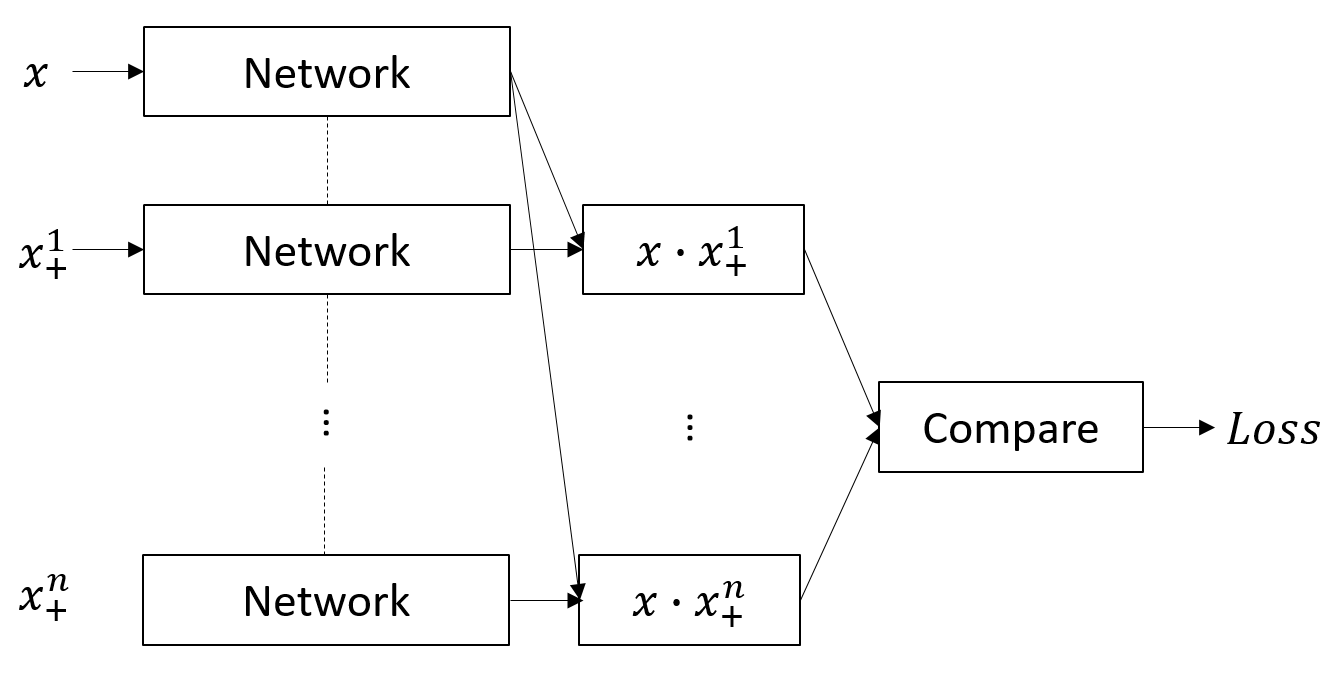
\includegraphics[width=0.7\linewidth]{../report_shaoheng/tuple_struct}
			\captionof{figure}{\color{Green} Structure of n-Tuple Network.}
		\end{center}\vspace{1cm}
		\begin{equation}
		L(\{x_i,x_i^+\}^N_{i=1})=\frac{1}{N}\log(\sum_{i=1}^N\exp(\sum_{j=1}^Ny^T_iy_j^+-y_i^Ty_i^+))  \label{eq:n-pair}
		\end{equation}
		
		\nocite{*} % Print all references regardless of whether they were cited in the poster or not
		\bibliographystyle{plain} % Plain referencing style
		\bibliography{../report_shaoheng/egbib} % Use the example bibliography file sample.bib
		
		
		\section*{Implementations}
		To facilitate our experiment, we write a wrapper class \verb|Network| for convolutional network, which provides three member functions \verb|add_conv()|, \verb|add_fc()| and \verb|connect()|. The implementation of a Triplet Network is as easy as follows.
		\begin{verbatim}
		net = Network(28, 28, 1, 2);
		net.add_conv(5, 5, 2, 2, 32);    net.add_conv(5, 5, 2, 2, 64);
		net.add_fc(1024);                net.add_fc(256);
		mid_output = net.connect(mid_input);
		pos_output = net.connect(pos_input);
		neg_output = net.connect(neg_input);
		\end{verbatim}
		However, the implementation of loss functions still needs hard work.
		\section*{Results}
		The Siamese Network can separate the classes fairly. Interesting overlappings between digits ``9'', ``7'' and ``4'' and between digits ``2'' and ``3'' is observed. In Triplet Network, these overlappings are further suppressed, which leads to a better separation.
		\begin{center}\vspace{1cm}
			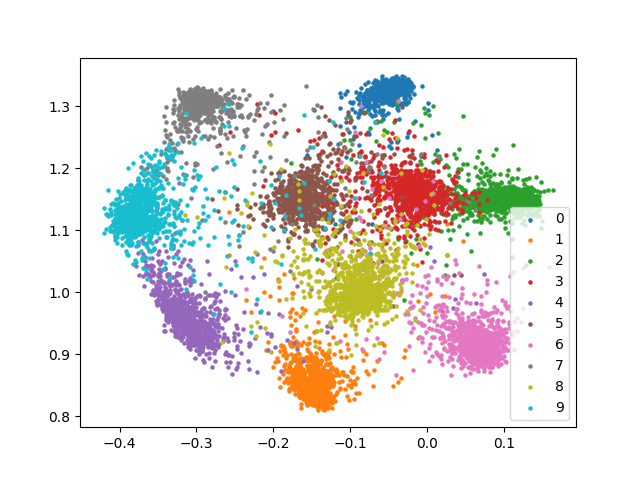
\includegraphics[width=0.45\linewidth]{../report_shaoheng/siamese}
			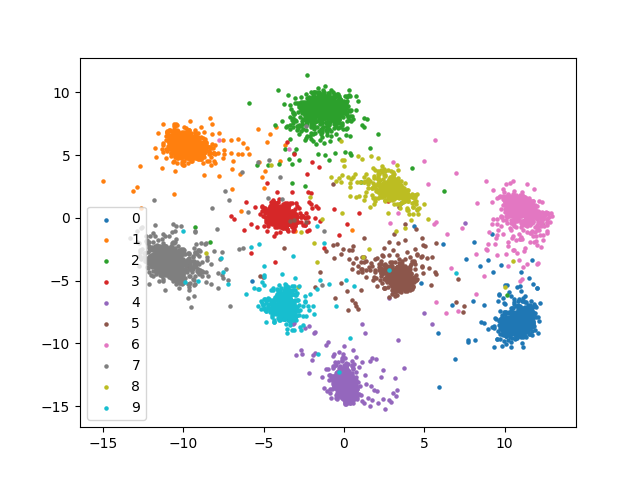
\includegraphics[width=0.45\linewidth]{../report_shaoheng/triplet}
			\captionof{figure}{\color{Green} Left: Siamese Network; Right: Triplet Network}
		\end{center}\vspace{1cm}
		
		The original network is impaired by a trivial all zero solution for dot product. As a result, all points shrinks to a very small area. Modified loss function involves the L2-Norm, which resolves the shrinking problem, but does not lead to a better separation.
		\begin{equation}
		Loss(\{x_i,x_i^+\}^N_{i=1})\notag
		=\frac{1}{N}\log(\sum_{i=1}^N\exp(\sum_{j=1}^Ny^T_iy_j^+-y_i^Ty_i^+))+ \frac{\lambda}{2N} \sum_{i=1}^N(\lVert y_i\rVert^2+ \lVert y^+_i\rVert^2)
		\end{equation}
		
		\begin{center}\vspace{1cm}
			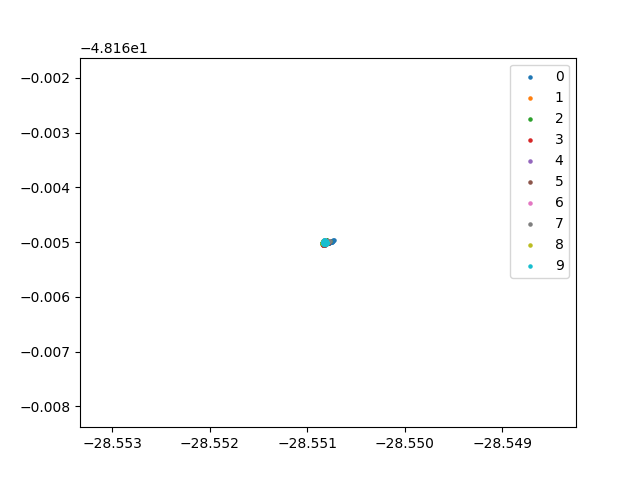
\includegraphics[width=0.45\linewidth]{../report_shaoheng/fail_tuple}
			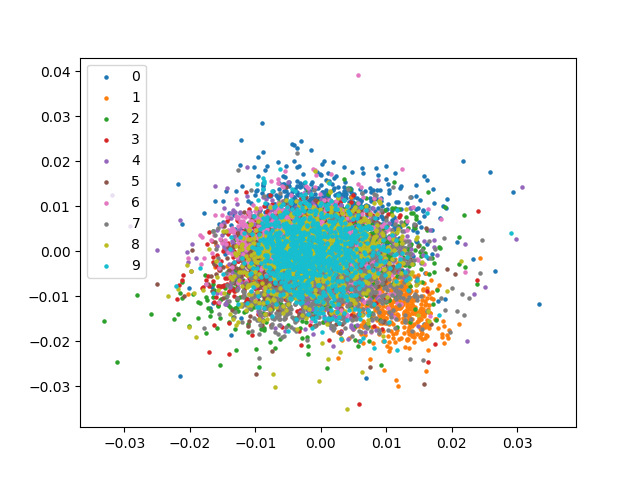
\includegraphics[width=0.45\linewidth]{../report_shaoheng/fig150}
			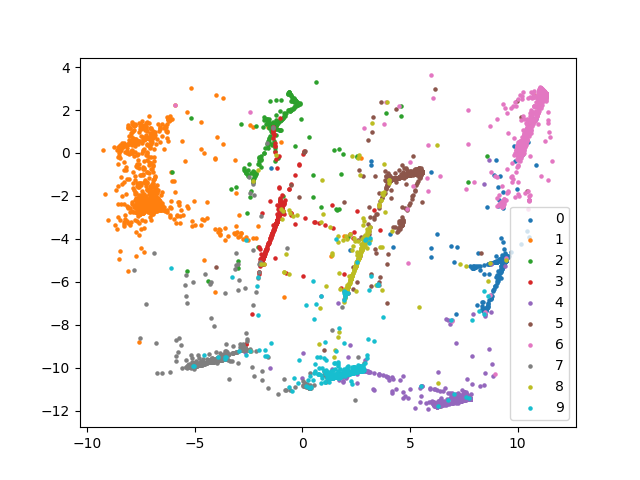
\includegraphics[width=0.45\linewidth]{../report_shaoheng/first_tuple}
			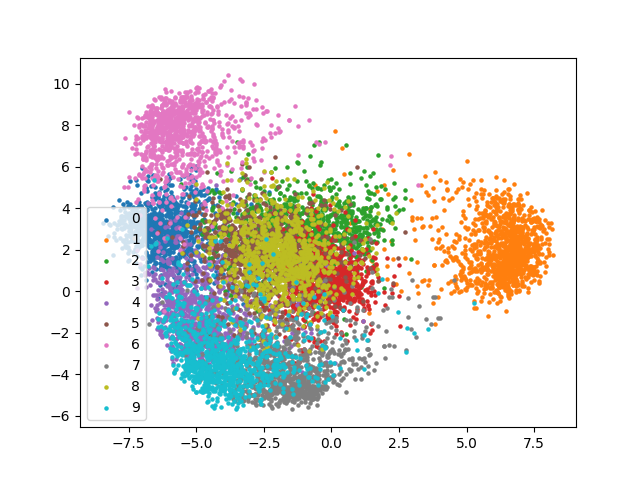
\includegraphics[width=0.45\linewidth]{../report_shaoheng/second_tuple}
			\captionof{figure}{\color{Green} Top left: Original n-Tuple Network; Top right: n-Tuple Network with L2 Norm\\ Bottom left: n-Tuple Network with Triplet loss; Bottom right: n-Tuple Network with modified Triplet loss}
		\end{center}\vspace{1cm}
		
		We directly use loss function on n-Tuple framework, which gives 90 triplets per 20 images, and produces a well separated but badly scattered figure. The reason may be the high dependency of the triplets. We designed a new loss function resembles the Triplet Network loss function but combines all 10 classes into one expression. As a result, the scattering is better but the separation is worse.
		\begin{equation}
		Loss = \frac{\exp{(\lvert y-y_+ \rvert)}}{\exp{(\lvert y-y_+ \rvert)} + \sum_i\exp{(\lvert y-y_-^i \rvert)}}
		\end{equation}
		%----------------------------------------------------------------------------------------
		%	CONCLUSIONS
		%----------------------------------------------------------------------------------------
		
		\color{SaddleBrown} % SaddleBrown color for the conclusions to make them stand out
		
		\section*{Conclusions}
		
		\begin{itemize}
			\item Our wrapper class gives a good basis for metric learning experiments.
			\item The Siamese Network and Triplet Network perform as expected. Triplet Network outperforms Siamese Network by reduce overlapping of digits that are easily get confused.
			\item We are not able to reproduce the original n-Tuple Network, but we designed multiple loss function as partial fixes.
		\end{itemize}
		
		\color{DarkSlateGray} % Set the color back to DarkSlateGray for the rest of the content
		
		%----------------------------------------------------------------------------------------
		%	FORTHCOMING RESEARCH
		%----------------------------------------------------------------------------------------
		
		\section*{Future Research}
		
		\begin{itemize}
			\item Show quantitative comparison of the methods, although the difference performance is intuitive.
			\item Combine the loss functions for n-Tuple to balance the scattering and the separation, or find new loss functions to get a better performance.
		\end{itemize}
		
	\end{multicols}
\end{document}